\documentclass[twoside]{article}%
\usepackage[T1]{fontenc}%
\usepackage[utf8]{inputenc}%
\usepackage{lmodern}%
\usepackage{textcomp}%
\usepackage{lastpage}%
\usepackage{parskip}%
\usepackage[top=1in,lmargin=.5in,rmargin=.5in]{geometry}%
\usepackage{subfig}%
\usepackage{tkz-euclide}%
\usepackage{tikz}%
\usepackage{fancyhdr}%
%
\fancypagestyle{header}{ 
\renewcommand{\headrulewidth}{0pt}%
\renewcommand{\footrulewidth}{0pt}%
\fancyhead{ 
}%
\fancyfoot{ 
}%
\fancyhead[L]{ 
Name:%
\linebreak%
SDFfSDsdfd
}%
\fancyhead[R]{ 
Date: 
}
}%
%
\begin{document}%
\normalsize%
\setlength{\floatsep}{1.0pt plus 5.0pt minus 2.0pt}%
\setlength{\intextsep}{1.0pt plus 5.0pt minus 2.0pt}%
\setlength{\textfloatsep}{1.0pt plus 5.0pt minus 2.0pt}%
\setcounter{topnumber}{10}%
\setcounter{bottomnumber}{10}%
\setcounter{totalnumber}{10}%
\makeatletter%
\setlength{\@fptop}{0pt}%
\setlength{\@fpbot}{0pt plus 1fil}%
\makeatother%
\usetikzlibrary{calc}%
\pagestyle{header}%
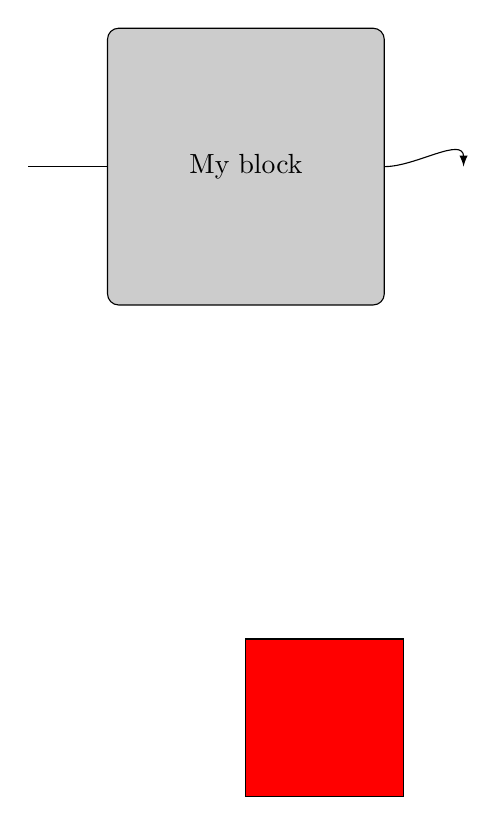
\begin{tikzpicture}%
\node[draw,rounded corners,align=center,minimum size=100pt,fill=black!20] (box) {My block};%
\path[draw,fill=red] (0.0,-6.0) rectangle (2.0,-8.0);%
\path[draw] (box.west) -- ++(-1.0,0.0);%
\path[draw] (box.east) edge[-latex,in=90,out=0] ++(1.0,0.0);%
\end{tikzpicture}%
When solving the equation 2(2x^2+5)-6=5x^2+2, Joe wrote 2(2x^2+5)=5x^2+8, as their first step. Which property justifies Joe's first step%
(1) Addition property of equality%
\vspace*{.05in}%
\newline%
\vspace*{.05in}%
(2) Distributive property of equality%
\newline%
\vspace*{.05in}%
(3) Multiplication property of equality%
\newline%
\vspace*{.05in}%
(4) Commutative property of equality%
Hid from you%
\end{document}